\newcommand{\institut}{Institut f\"ur Energie und Automatisiertungstechnik}
\newcommand{\fachgebiet}{Elektronische Mess- und Diagnosetechnik}
\newcommand{\veranstaltung}{Praktikum Messdatenverarbeitung}
\newcommand{\pdfautor}{Dirk Babendererde (321 836), Thomas Kapa (325 219), Magdalene Busuru (319 433)}
\newcommand{\autor}{Dirk Babendererde (321 836)\\ Thomas Kapa (325 219)\\ Magdalene Busuru (319 433)}
\newcommand{\pdftitle}{Praktikum Messdatenverarbeitung Termin 1}
\newcommand{\prototitle}{Praktikum Messdatenverarbeitung \\ Termin 1}
\newcommand{\aufgabe}{}


\newcommand{\gruppe}{Gruppe: G2 Fr 08-10}
\newcommand{\betreuer}{Betreuer: J\"urgen Funk}



\input{../../../packages/tu_header_8}



% \lstlistoflistings
\definecolor{darkgray}{rgb}{0.95,0.95,0.95}
\lstset{language=Scilab}
\lstset{inputencoding=utf8}
%\lstset{extendedchars=true} % Umlaute an der richtigen stelle und nicht am Anfang ausgeben
\lstset{backgroundcolor=\color{darkgray}}
\lstset{numbers=left, numberstyle=\tiny, stepnumber=1, numbersep=7pt, breaklines=true}
\lstset{keywordstyle=\color{red}\bfseries\emph}
\lstset{
breaklines,
numbers=left,
frame=single,
xleftmargin=-2cm,
xrightmargin=-1.5cm
}
% enables UTF-8 in source code: (dirty, dirty hack)
\lstset{literate=
    %Deutsch
    {ä}{{\"a}}1 {ö}{{\"o}}1 {ü}{{\"u}}1 {Ä}{{\"A}}1 {Ö}
    {{\"O}}1 {Ü}{{\"U}}1 {ß}{\ss}1
    %Türkisch
    {â}{{\^{a}}}1 {Â}{{\^{A}}}1 {ç}{{\c{c}}}1 {Ç}{{\c{C}}}1 {ğ}{{\u{g}}}1 {Ğ}{{\u{G}}}1 {ı}{{\i}}1 {İ}{{\.{I}}}1 {ö}{{\"o}}1 {Ö}{{\"O}}1 {ş}{{\c{s}}}1
    {Ş}{{\c{S}}}1 {ü}{{\"u}}1 {Ü}{{\"U}}1
    %Polish
    {ą}{{\k{a}}}1 {ć}{{\'c}}1 {ę}{{\k{e}}}1 {ł}{{\l{}}}1 {ń}{{\'n}}1 {ó}{{\'o}}1 {ś}{{\'s}}1 {ż}{{\.z}}1 {ź}{{\'z}}1 {Ą}{{\k{A}}}1 {Ć}{{\'C}}1
    {Ę}{{\k{E}}}1 {Ł}{{\L{}}}1 {Ń}{{\'N}}1 {Ó}{{\'O}}1 {Ś}{{\'S}}1 {Ż}{{\.Z}}1 {Ź}{{\'Z}}1
    %Spanish
    {á}{{\'a}}1 {é}{{\'e}}1 {í}{{\'i}}1 {ó}{{\'o}}1 {ú}{{\'u}}1 {ñ}{{\~n}}1
}

%     \lstinputlisting{./praktikum6.sce}

%---------------------------------------------------------------------
%---------------------------------------------------------------------
%---------------------------------------------------------------------

\section{Vorbereitungsaufgaben}


\bq

Eine digitale Messkette besteht aus einem Sensor, der Signalkonditionung (z.B.
Linearisierung, Verstärkung \ldots), dem Antialiasingfilter, einem Abtast- und
Halteglied und einem Analog-Digital-Umsetzer.
Der Analog-Digital-Umsetzer hat eine minimale Abtastfrequenz, z.B. dadurch, dass
man ein Register als Referenz für einen Timer nutzt, dass aber eine begranzte
Anzahl an Bits zur Verfügung stellt.
Sensor, Signalkonitionierung und Antialiasingfilter sitzen in der Wandlerbox,
Abtast- und Haltglied und ADU sitzen auf dem Microcontroller.
\section{Vorbereitung}
\begin{quote}
    
    \subsection{Tiefpassfilter 2. Ordnung}
    \begin{quote}
        
        Um die Dämpfung bestimmen zu können muss zunächst das $U_{LSB}$ errechnet werden:
        \begin{equation}
    	\begin{split}
    		U_{LSB} = \frac{14V}{2^{10} - 1 Bit} = \frac{14V}{1023 Bit}
    	\end{split}
        \end{equation}
        
        Die Dämpfung ergibt sich nun daraus, dass, aber der Grenzfrequenz, die Maximale Eingangsspannung von $\pm 7V$ auf unter $U_{LSB}$ gedämpft
        werden muss.
        Daraus folgt:
        
        
        \begin{equation}
    	\begin{split}
    		A = \frac{14}{7} \p \frac{1}{1023} = \frac{2}{1023} = -27,1 dB
    	\end{split}
        \end{equation}
        
        
        Nun simulieren wir einen Butterworth-Tiefpass 2. Ordnung und lesen ab, ab felcher Frequenz die Amplitude unter $-27,1 dB$ sinkt.
        
        %2 Grafiken:
        \begin{center}
        \vspace{-1.5cm}
        \begin{tabular}{ll}
        
        \hspace{-4.5cm}
            \begin{minipage}{0.6\textwidth}
                
                \begin{figure}[H]
                    \label{fig:butter_2} 
                    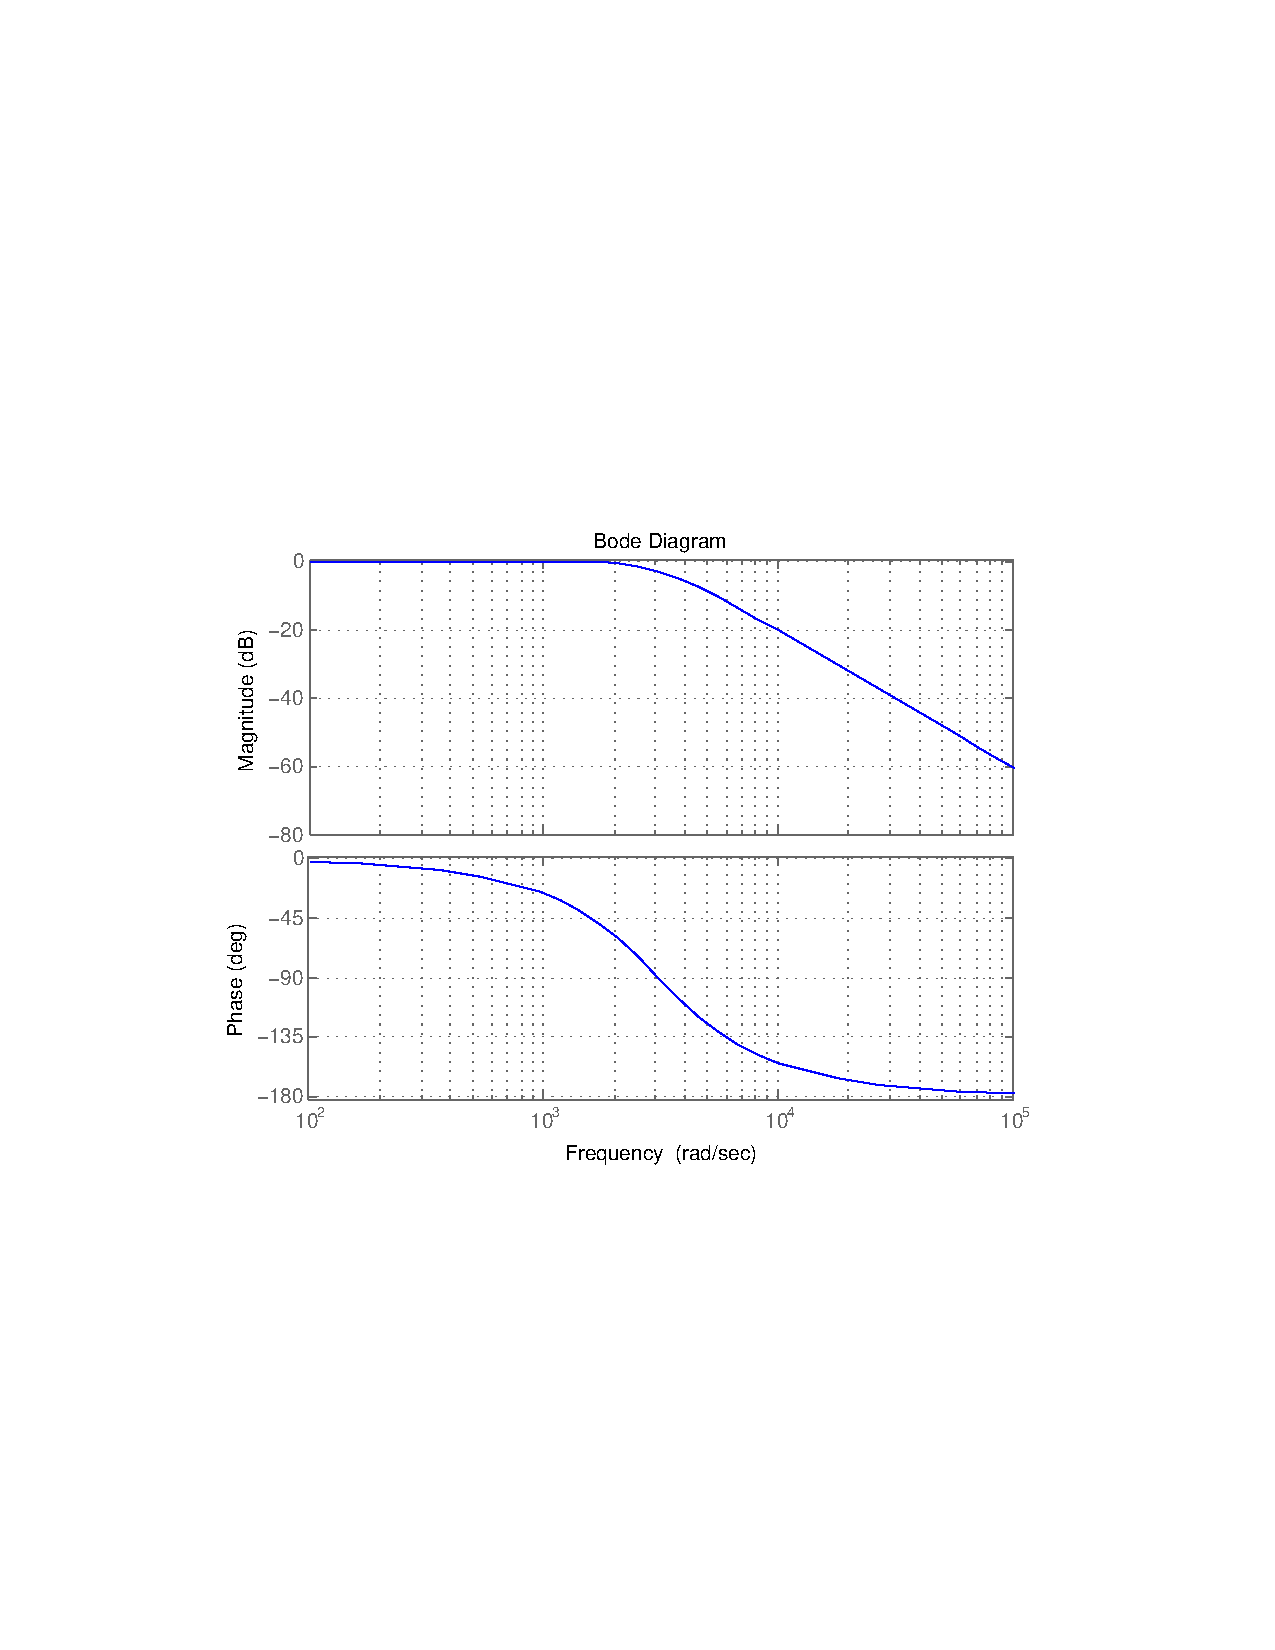
\includegraphics[scale=0.7, trim = 3.5cm 7cm 3.5cm 7cm, clip]{Bilder/butter_2} %FIXME [width=640px, height=474px]
                    \caption{Butterworth Filter 2. Ordn.}
                \end{figure}

            \end{minipage}
        
            \begin{minipage}{0.6\textwidth}
                \begin{figure}[H]
                    \label{fig:butter_2}
                    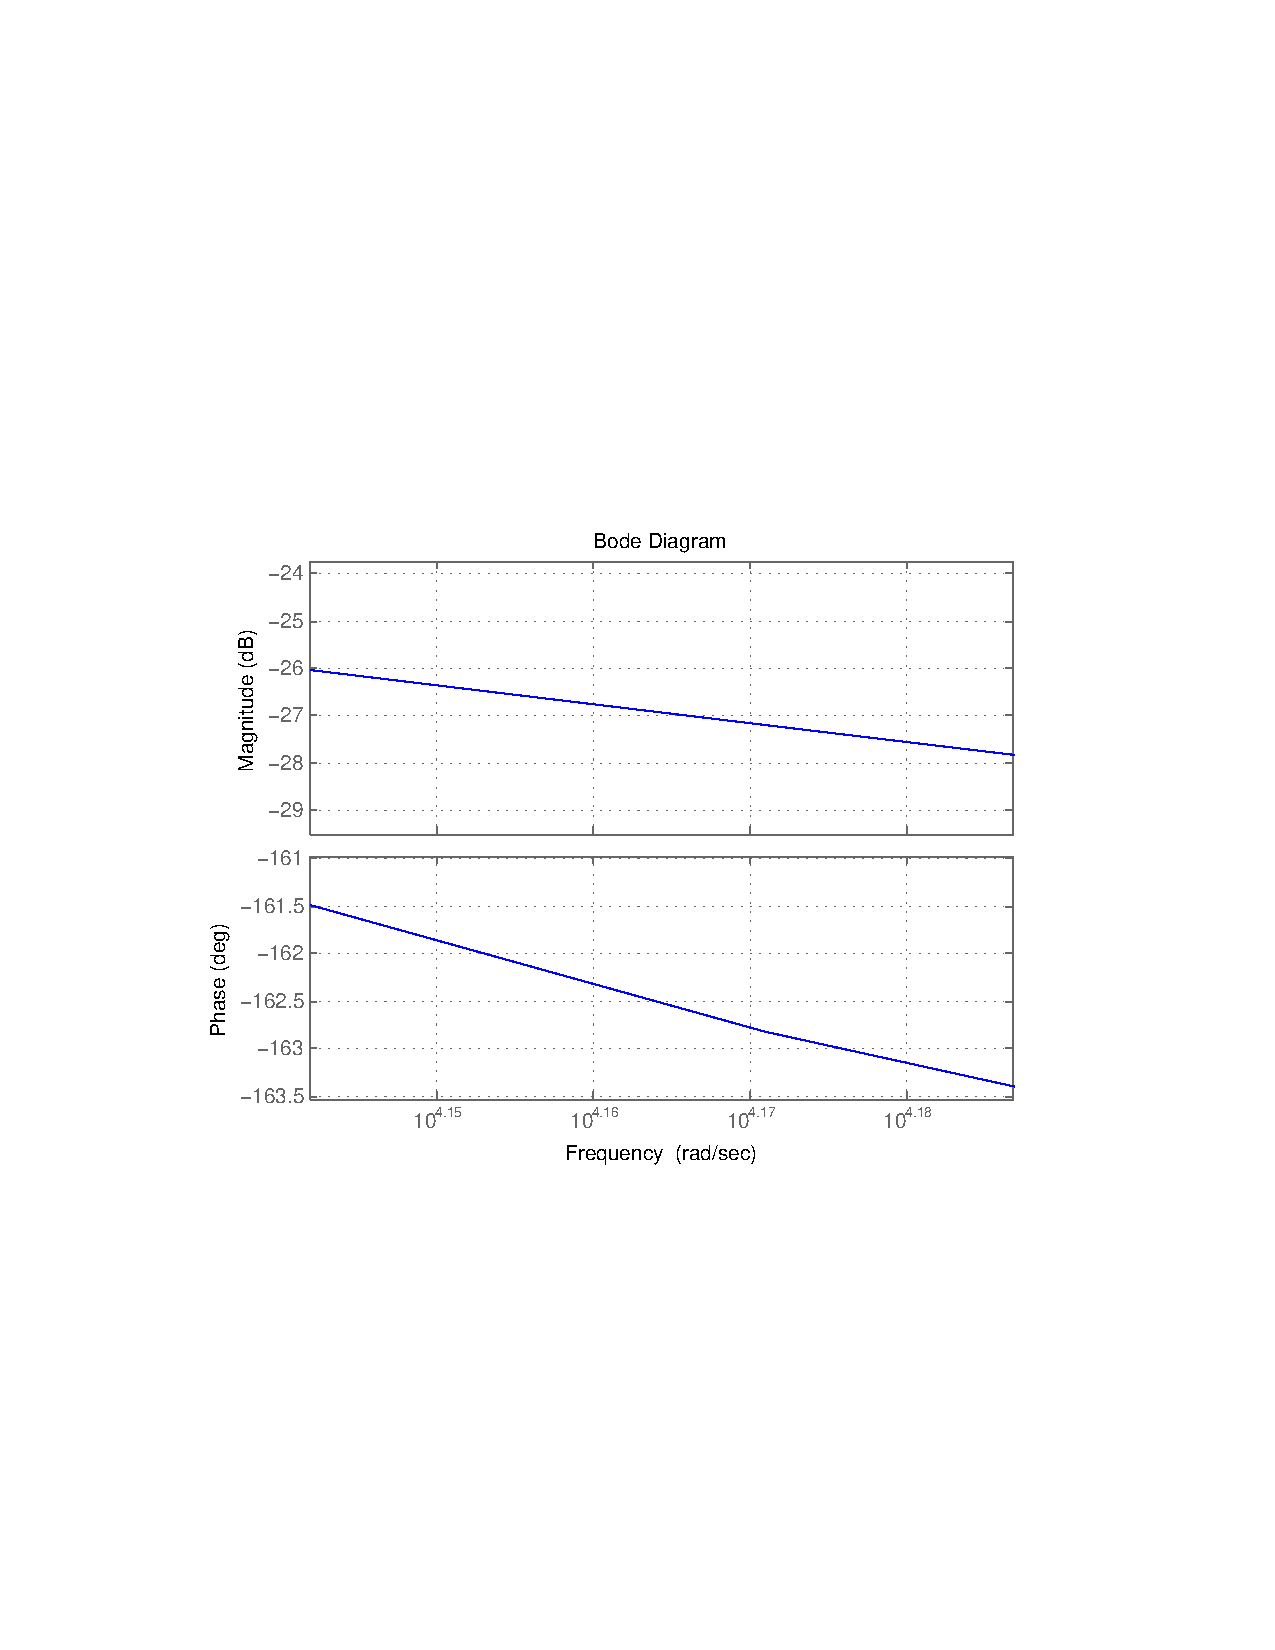
\includegraphics[scale=0.7, trim = 3.5cm 7cm 3.5cm 7cm, clip]{Bilder/butter_2_zoom} %FIXME [width=640px, height=474px]
                    \caption{In die Grafik des Filters hineingezoomt}
                \end{figure}
            \vspace{-0.4cm}
                                    
            \end{minipage}
        
        \end{tabular}
        \end{center}
            
        \vspace{1.5 cm}    
        Daraus folgt, dass $f \approx 14,8 kHz$.\\
        Da $f_0 < 2 \p f$ sein muss, ist die mindestabtastrate:\\
         
        \begin{equation}
    	\begin{split}
            f_0 \approx 2 \p 14,8 kHz = 29,6 kHz
    	\end{split}
        \end{equation}
    \end{quote}



    \subsection{Tiefpassfilter 2. Ordnung}
    \begin{quote}
        
        Die Vorgehensweise beim Tiefpass 8. ordnung ist analog.
        
        
        %2 Grafiken:
        \begin{center}
        \vspace{-1.5cm}
                
        \end{center}
        \begin{tabular}{ll}
        
        \hspace{-4.5cm}
            \begin{minipage}{0.6\textwidth}
                
                \begin{figure}[H]
                    \label{fig:butter_2} 
                    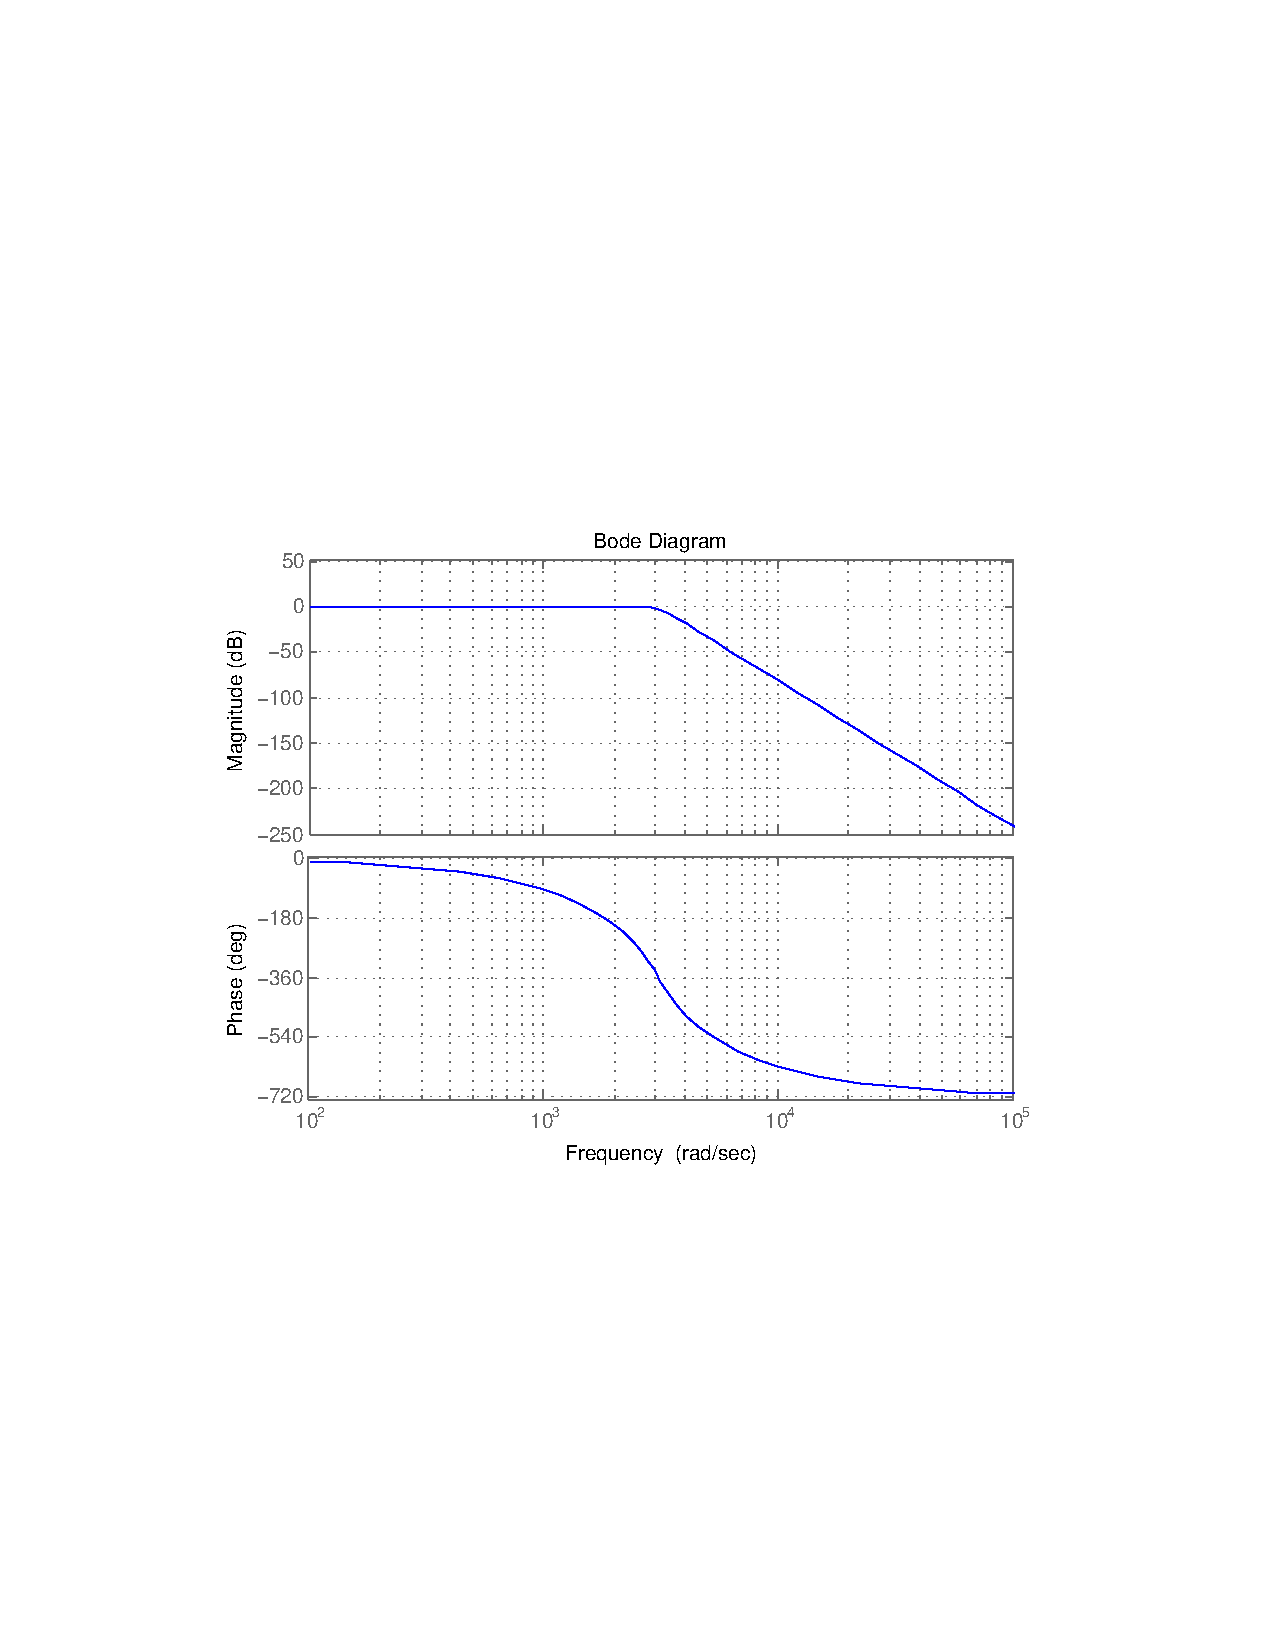
\includegraphics[scale=0.7, trim = 3.5cm 7cm 3.5cm 7cm, clip]{Bilder/butter_8} %FIXME [width=640px, height=474px]
                    \caption{Butterworth Filter 2. Ordn.}
                \end{figure}

            \end{minipage}
        
            \begin{minipage}{0.6\textwidth}
                \begin{figure}[H]
                    \label{fig:butter_2}
                    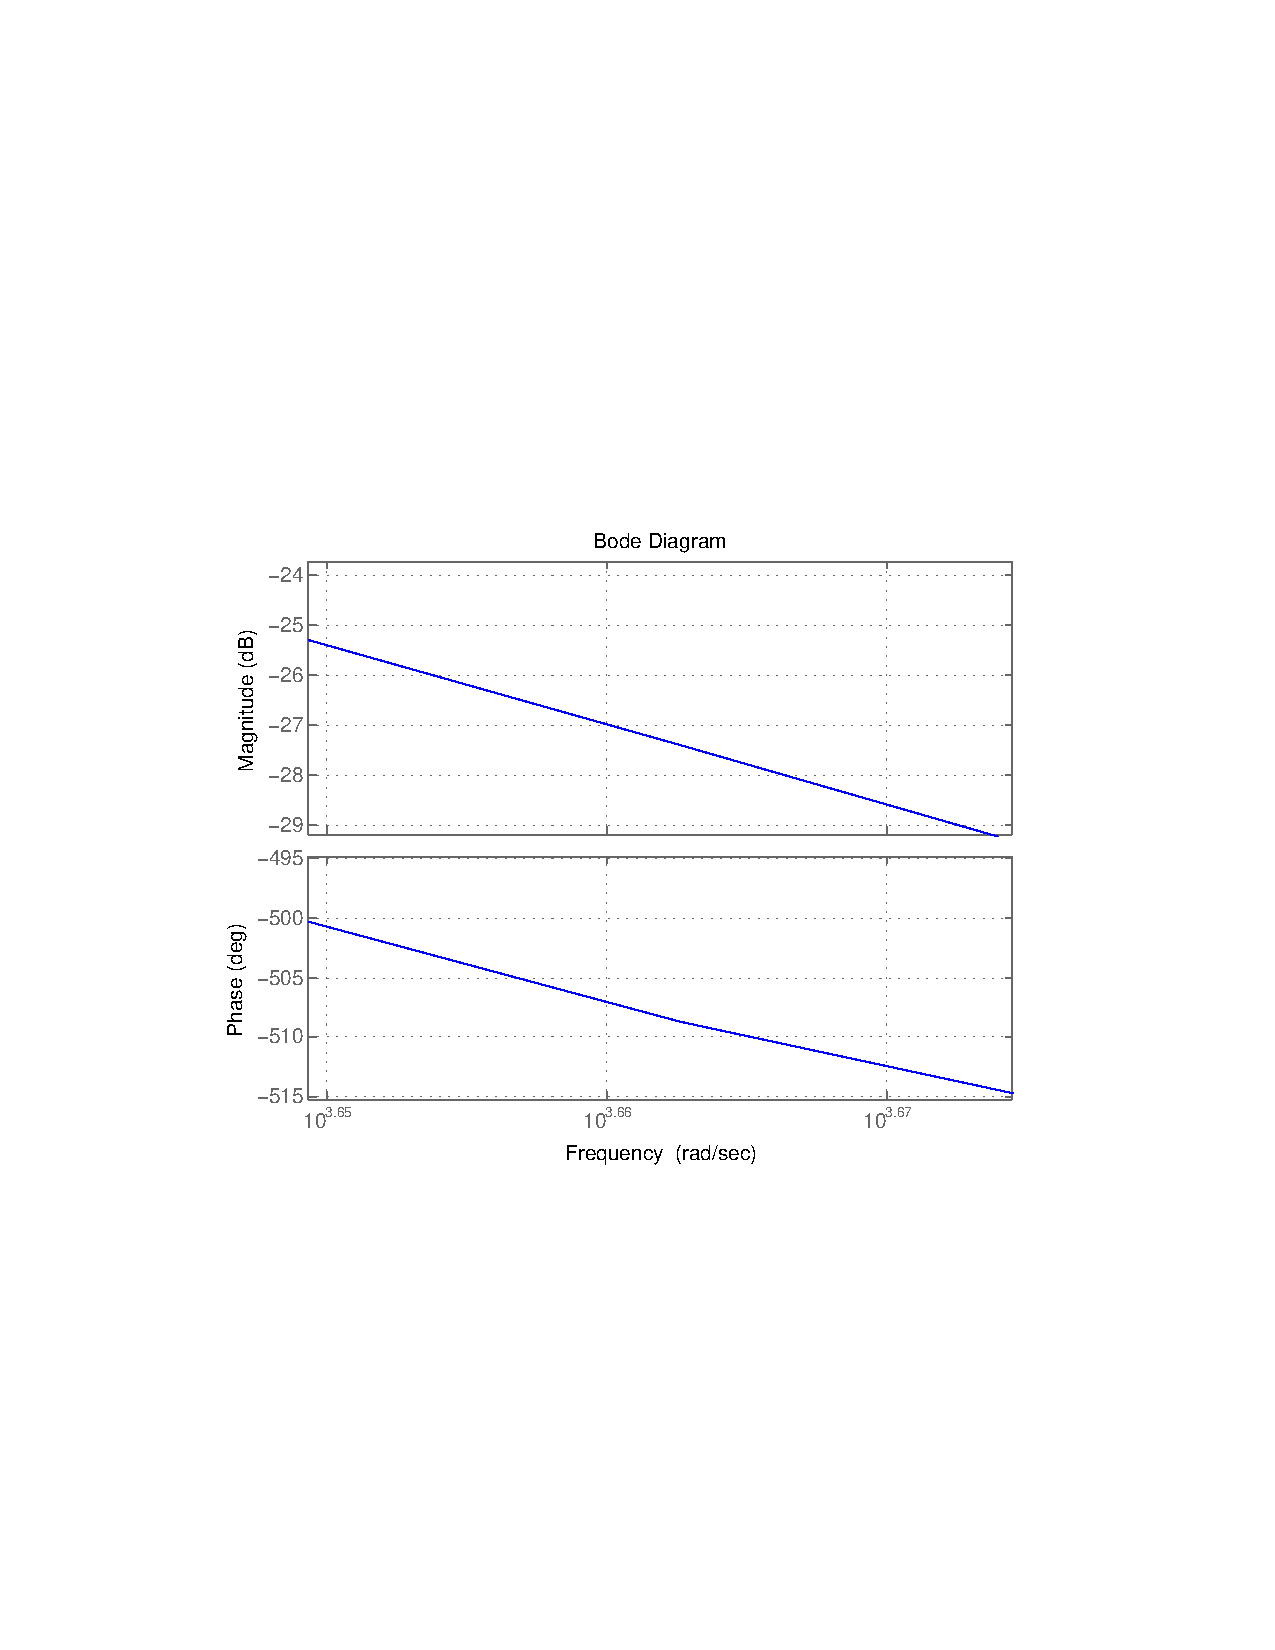
\includegraphics[scale=0.7, trim = 3.5cm 7cm 3.5cm 7cm, clip]{Bilder/butter_8_zoom} %FIXME [width=640px, height=474px]
                    \caption{In die Grafik des Filters hineingezoomt}
                \end{figure}
            \vspace{-0.4cm}
                                    
            \end{minipage}
        
        \end{tabular}
        \end{center}
    \end{quote}

    \begin{equation}
    \begin{split}
        f_0 \approx 2 \p 4,6 kHz = 9,2 kHz
    \end{split}
    \end{equation}
    

    
\end{quote}



\eq

\end{document}
